\section{Introduction}

The human brain is the subject of intense research, a significant portion of
which relies on simulations of large-scale models of the brain. Due to the
unusual computational requirements of these simulations, numerous specialised
hardware platforms have been developed to cope
\cite{furber07,moore12,maguire07,choudhary12,misra10}. This project will focus
on the interconnection networks within such systems, in particular on network
topology and power management.

Neural models of the brain typically consist of a directed graph of `neurons'
with simple, well defined behaviours and which communicate by sending `spikes'
to their neighbours. The only significant features of a spike are its origin and
time of arrival. Such models have been demonstrated to reproduce high-level
cognitive behaviours such as problem solving and memory \cite{eliasmith12}. 

Conventional super computer interconnection networks are poorly suited to human
scale models containing tens of billions of neurons \cite{williams88} each with
thousands of connections \cite{kung88}. These networks are designed to handle
the transmission of large blocks of data to a limited set of destinations, in
sharp contrast with neural simulation requirements. A spike may be sent to
thousands of destinations and requires only an origin ID and timestamp to be
transmitted. In realtime simulations a timestamp is not required though maximum
latency must be strictly limited. Due to this mismatch, alternative technologies
are popular in neural simulators. Recent systems, such as SpiNNaker
\cite{furber07} and Bluehive \cite{moore12}, have begun to incorporate
super-computer style interconnect to benefit from increased speed at the expense
of power. It is here that this project hopes to contribute to a new generation
of power efficient interconnection network.

\section{SpiNNaker}
	
	\begin{figure}
		\center
		\begin{tikzpicture}[thick]
	
	\pgfmathsetlengthmacro{\sep}{2.5em}
	
	\pgfmathsetlengthmacro{\labelsep}{0.5em}
	\tikzset{widelabel/.style={ font=\footnotesize
	                      , align=center
	                      , inner sep=0
	                      }}
	\tikzset{label/.style={ widelabel
	                      , text width=3cm
	                      }}
	
	
	% Callout from #1 to callout box #2 from corner #3 to #4 and corner
	% #5 to #6
	\tikzset{glow/.style={line width=1.0mm,white}}
	\newcommand{\callout}[6]{
		\draw [glow] (#2.north west) rectangle (#2.south east);
		\draw [glow] (#1.#3) -- (#2.#4);
		\draw [glow] (#1.#5) -- (#2.#6);
		
		\draw        (#2.north west) rectangle (#2.south east);
		\draw        (#1.#3) -- (#2.#4);
		\draw        (#1.#5) -- (#2.#6);
	}
	
	\newcommand{\hcallout}[2]{
		\callout{#1}{#2}{north east}{north west}{south east}{south west}
	}
	\newcommand{\vcallout}[2]{
		\callout{#1}{#2}{south east}{north east}{south west}{north west}
	}
	
	% A mess of neurons
	\node (neurons) [inner sep=0]
	      {\input{|"python2 figures/random-network.py 10 25 25 5 0.2 100 3 0.2 1.0"}}
	      ;
	
	% A SpiNNaker die
	\node (die) [inner sep=0]
	      [right=\sep of neurons]
	      {\includegraphics[height=3cm]{figures/spinnakerDie}};
	\node (core) at ([shift={(5.0mm,1.5mm)}]die.west)
	      [ inner sep=0
	      , minimum width =7mm
	      , minimum height=5mm
	      ]
	      {};
	\hcallout{neurons}{core}
	
	% A SpiNNaker board
	\node (board) [inner sep=0]
	      [right=\sep of die]
	      {\includegraphics[height=3cm]{figures/spinnakerBoard}};
	\node (chip) at ([shift={(5.0mm,1.6mm)}]board.west)
	      [ inner sep=0
	      , minimum width =3mm
	      , minimum height=3mm
	      ]
	      {};
	\hcallout{die}{chip}
	
	% A rack of boards
	\node (rack) [inner sep=0]
	      [right=\sep of board]
	      {\includegraphics[height=3cm]{figures/spinnakerRack}};
	\node (fitted board) at ([shift={(7mm,2mm)}]rack.west)
	      [ inner sep=0
	      , minimum width =1mm
	      , minimum height=16mm
	      ]
	      {};
	\hcallout{board}{fitted board}
	
	% A ten cabinet machine
	\coordinate (top row) at ($(neurons.south west)!0.5!(rack.south east)$);
	\node (cabinet) [inner sep=0]
	      [below=\sep of top row]
	      {\includegraphics[width=\textwidth]{figures/spinnaker106}};
	\node (fitted rack) at ([shift={(-23.2mm,-5.5mm)}]cabinet.north east)
	      [ inner sep=0
	      , minimum width =11.5mm
	      , minimum height=6.5mm
	      ]
	      {};
	\vcallout{rack}{fitted rack}
	
	% Labels
	\node [above=\labelsep of neurons, label] {1,000 neurons \\ per core.};
	\node [above=\labelsep of die, label] {18 cores \\ per chip.};
	\node [above=\labelsep of board, label] {48 chips \\ per board.};
	\node [above=\labelsep of rack, label] {24 boards \\ per rack.};
	\node [below=\labelsep of cabinet, widelabel] {5 racks per cabinet, 10
	cabinets.};
	
\end{tikzpicture}


		
		\caption{Construction of the largest planned SpiNNaker machine.}
		\label{fig:spinnaker-abstractions}
	\end{figure}
	
	SpiNNaker is a hardware platform which combines low-power mobile-phone grade
	CPU cores using a custom, high-performance interconnection network to simulate
	large networks of neurons in realtime. The largest planned machine, which is
	in the final stages of manufacturing, is designed to simulate one billion
	($10^9$) neurons in biological realtime \cite{navaridas09} and will fill ten
	server-room cabinets as described in figure \ref{fig:spinnaker-abstractions}.
	
	Between chips on the same board asynchronous, parallel signalling is used with
	groups of 16 wires required to communicate data between neighbouring chips
	\cite{bainbridge02}. This technique only consumes energy when the link is in
	use. Connecting this many wires between different boards would be
	prohibitively expensive so a different technology, High-Speed Serial (HSS), is
	used \cite{athavale05}. HSS links can support high bandwidths and in
	SpiNNaker, one board-to-board HSS link carries the load of eight asynchronous
	links.  Unfortunately, HSS links consume energy at the same rate when loaded
	and idle; to reduce power the links must be operated at a lower speed.
	
	In conventional HSS applications, links change speed dynamically depending on
	load \cite{infinibandta08} to cope with unpredictable traffic patterns as in
	neural simulations. Unfortunately, during link speed changes, HSS links become
	non-operational for around 1 ms \cite{xilinx14}. To maintain realtime
	performance in SpiNNaker, the maximum latency for a spike traversing the
	network is also around 1 ms making delays during link speed changes
	unacceptable. Because of this HSS links in SpiNNaker and other simulators are
	operated at full speed at all times despite average network loads of between
	5\% and 10\% \cite{moore12,navaridas09} link capacity.
	
	% XXX Why are the project goals being introduced as new again?
	This project hopes to develop a new architecture for neural simulator
	interconnection networks which both allows link speed changes without breaking
	simulations and while also further reducing the network load. Since
	SpiNNaker's HSS board-to-board links are implemented by reconfigurable FPGAs
	the platform lends itself to a prototype implementation.

\section{Preliminary work}
	
	Work has initially focused on developing improvements to neural
	interconnection networks and building infrastructure to enable implementation
	of such improvements within SpiNNaker.
	
	\subsection{SpiNNaker interconnect modelling}
		
		A detailed simulation model of SpiNNaker's interconnect was developed and
		compared with SpiNNaker hardware as part of a collaborative work exploring
		novel hardware-accelerated modelling of computer architectures. The result
		demonstrated a strong correspondence between the simulator and SpiNNaker
		indicating its suitability for use in the development of improvements to
		SpiNNaker's interconnect. This work is being prepared for journal submission
		in early September.
	
	\subsection{Wiring large systems with small-world connectivity}
		
		\begin{figure}
			\center
					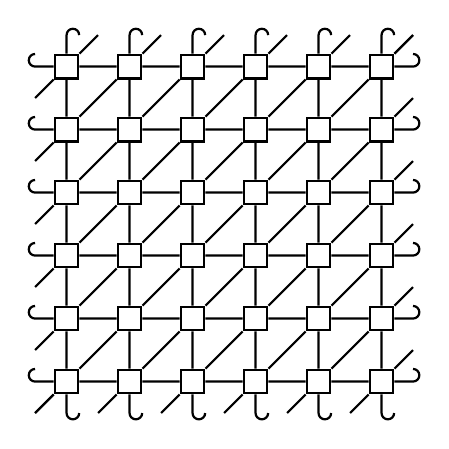
\begin{tikzpicture}[thick,scale=0.80]
			
			\def\width{6}
			\def\height{6}
			\pgfmathtruncatemacro{\widthh}{\width - 1}
			\pgfmathtruncatemacro{\heightt}{\height - 1}
			
			\def\lsize{0.1}
			\def\osize{0.5}
			
			\begin{scope}[minimum size=0.25cm,inner sep=0]
				\foreach \y in {1,...,\height}{
					\foreach \x in {1,...,\width}{
						\node (chip-\x-\y) at (\x,\y) [draw,fill=white,rectangle,minimum size=0.30cm,inner sep=0] {};
					}
				}
			\end{scope}
			
			% The obvious internal links
			\foreach \y in {1,...,\heightt}{
				\foreach \x in {1,...,\widthh}{
					\pgfmathtruncatemacro{\xx}{\x+1}
					\pgfmathtruncatemacro{\yy}{\y+1}
					\draw (chip-\x-\y) -- (chip-\xx-\yy);
					
					\pgfmathtruncatemacro{\xx}{\x+1}
					\pgfmathtruncatemacro{\yy}{\y+0}
					\draw (chip-\x-\y) -- (chip-\xx-\yy);
					
					\pgfmathtruncatemacro{\xx}{\x+0}
					\pgfmathtruncatemacro{\yy}{\y+1}
					\draw (chip-\x-\y) -- (chip-\xx-\yy);
				}
			}
			
			% The non-loop upper/right links
			\foreach \y in {1,...,\heightt}{
				\pgfmathtruncatemacro{\yy}{\y+1}
				\draw (chip-\width-\y) -- (chip-\width-\yy);
			}
			\foreach \x in {1,...,\widthh}{
				\pgfmathtruncatemacro{\xx}{\x+1}
				\draw (chip-\x-\height) -- (chip-\xx-\height);
			}
			
			% The looping left/right links
			\foreach \y in {1,...,\height}{
				\draw 
					(chip-\width-\y) -- ++(\osize,0) arc (-90:90:\lsize);
				\draw  (chip-1-\y) -- ++(-\osize,0) arc (90:-90:-\lsize);
			}
			
			% The looping up/down links
			\foreach \x in {1,...,\width}{
				\draw  (chip-\x-\height) -- ++(0,\osize) arc (180:0:\lsize);
				\draw  (chip-\x-1)       -- ++(0,-\osize) arc (-180:0:\lsize);
			}
			
			% The looping diagonal links
			\foreach \x in {1,...,\width}{
				\draw  (chip-\x-\height) -- ++(\osize,\osize);
				\draw  (chip-\x-1)       -- ++(-\osize,-\osize);
			}
			\foreach \y in {1,...,\height}{
				\draw  (chip-\width-\y) -- ++(\osize,\osize);
				\draw  (chip-1-\y)      -- ++(-\osize,-\osize);
			}
			
		\end{tikzpicture}

			
			\caption{2D hexagonal torus topology used in SpiNNaker. Each box is an
			eighteen core SpiNNaker chip. Links at the edges of the network
			wrap-around to connect to those on the other side. Actual networks are
			much larger.}
			\label{fig:spinn-topology}
		\end{figure}
		
		HSS technology imposes constraints on the lengths of wires used in large
		systems; for example in SpiNNaker, wires are limited to around 1 metre or
		less \cite{sata3spec}. SpiNNaker's network uses a 2D hexagonal torus
		topology (illustrated in figure \ref{fig:spinn-topology}) which, if laid out
		na\"ively, would require cables long enough to span the whole system. For
		the large machine in figure \ref{fig:spinnaker-abstractions}, this would be
		over 6 metres. Preliminary work has developed a tool to aid the design of
		alternative physical organisations of SpiNNaker machines (such as in the
		figure) which maintain the same logical connectivity but use wires of less
		than a metre.
		
		Watts and Strogatz demonstrated that adding a small number of random links
		to a torus topology can convert it into a `small-world' network
		\cite{watts98}. A well-known example of a small-world network is the human
		social network where the idea is popularly know as the theory of `six
		degrees of separation'. The theory states that any two people are connected
		by a chain of no more than six acquaintances. This property is also
		desirable in computer networks since it reduces the maximum and average
		number of `hops' messages must make when travelling through a network. This
		reduces both the latency of messages and also frees up resources on links
		\cite{shin11}. This freeing of resources enables the network to operate at
		lower speeds and thus lower power.
		
		Random links added to a network can easily require wires longer than a metre
		and allowing only short random connections was found to prevent the
		small-world effect from occurring. However, when systems were laid out to
		reduce wire lengths logically distant boards become physically close. This
		means that even short cables can create logically long connections.
	
	
	\subsection{High-speed serial (HSS)}
		
		Preliminary work has also resulted in the development of foundational
		hardware components for implementing new connectivity schemes within
		SpiNNaker's board-to-board interconnect. These components include a crossbar
		switch \cite{dally04} which allows spikes to be selectively redirected along
		links and interfaces for connecting links operating at different speeds.
		These components will be built upon during upcoming work.
		
		A proof of concept system was produced to demonstrate these components which
		connects SpiNNaker to a host PC using unused HSS connections. This prototype
		is intended to replace an existing Ethernet connection to SpiNNaker (which
		is out of the scope of this report) used for system management and
		interaction with neural models. Though the prototype link operates at a
		fraction of the maximum speed of an HSS link, it has achieved an
		order-of-magnitude improvement in host bandwidth for certain neural loads
		since it bypasses a software bottleneck in the Ethernet connectivity.


\section{Research plan}
	
	\begin{figure}
		\center
		\begin{tikzpicture}[thick,x=0.25cm]

%%%%%%%%%%%%%%%%%%%%%%%%%%%%%%%%%%%%%%%%%%%%%%%%%%%%%%%%%%%%%%%%%%%%%%%%%%%%%%%%
% Hacked-up Gantt Library
%%%%%%%%%%%%%%%%%%%%%%%%%%%%%%%%%%%%%%%%%%%%%%%%%%%%%%%%%%%%%%%%%%%%%%%%%%%%%%%%

% An entry in the Gantt chart. Takes a label, start offset, length and slack.
% Also defines a pair of labels "[label] start" and "[label] end" which can be
% used for drawing dependency lines.
\newcommand{\ganttEntry}[4]{
	% Label
	\node (label)
				[below=1.5ex of label.south east,anchor=east,minimum height=1.7em]
				{#1}
				;
	\coordinate (gantt labels end) at (label.south east);
	
	% Box
	\draw [fill=white]
	      ([shift={(#2   ,-.9ex)}]label.north east) rectangle
	      ([shift={(#2+#3,0.9ex)}]label.south east);
	
	% The tips of the box
	\coordinate (#1 end)
	         at ([shift={(#2+#3,0.9ex)}]label.south east);
	\coordinate (#1 start)
	         at ([shift={(#2   ,-.9ex)}]label.north east);
	
	% Slack line
	\draw [ultra thick]
	      ([shift={(#2+#3,0)}]$(label.north east)!0.5!(label.south east)$)
	   -- ++(#4,0);
}

\newcommand{\ganttDep}[2]{
	\draw [->,red] (#1 end) -| (#2 start);
}

\newcommand{\ganttVSep}[2]{
	\draw [#2] ([shift={(#1,0)}]gantt labels start) -- ([shift={(#1,0)}]gantt labels end);
}

% A new gantt chart. Takes a list of x-offset/label/major-label tuples. For each
% tuple a line is created with x-offset from the previous line and the span is
% labelled with "label". If major-label given, a major label will be drawn
% centered over the previous entries up until the last major-label.
\newenvironment{gantt}[1]{
	% Start the list of labels
	\node (label) [white] {Ag};
	\coordinate (gantt labels start) at (label.north east);
	\def\periods{#1}
}{
	\begin{scope}[on background layer]
		% Thick line separating from labels
		\draw (gantt labels start) -- (gantt labels end);
		
		% Start of the area covered by a "major" label
		\coordinate (gantt maj label start) at (gantt labels start);
		
		\foreach \x/\lab/\mlab in \periods {
			\coordinate (next gantt labels start) at ([shift={(\x,0)}]gantt labels start);
			\coordinate (next gantt labels end)   at ([shift={(\x,0)}]gantt labels end);
			
			% Minor label
			\node at ($(gantt labels start) !0.5! (next gantt labels start)$)
			      [anchor=west,rotate=90]
			      {\lab}
			      ;
			
			% Separator
			\ifthenelse{\equal{\mlab}{}}{
				\draw [help lines] (next gantt labels start) -- (next gantt labels end);
			}{
				\draw [help lines,thick] (next gantt labels start) -- (next gantt labels end);
			}
			
			\coordinate (gantt labels start) at (next gantt labels start);
			\coordinate (gantt labels end)   at (next gantt labels end);
			
			% Major label
			\ifthenelse{\equal{\mlab}{}}{}{
				\coordinate (next gantt maj label start) at (gantt labels start);
				\node at ($(gantt maj label start) !0.5! (next gantt maj label start)$)
				      [yshift=1cm,anchor=south]
				      {\mlab}
				      ;
				\coordinate (gantt maj label start) at (next gantt maj label start);
			}
		}
	\end{scope}
}



%%%%%%%%%%%%%%%%%%%%%%%%%%%%%%%%%%%%%%%%%%%%%%%%%%%%%%%%%%%%%%%%%%%%%%%%%%%%%%%%
% The Chart...
%%%%%%%%%%%%%%%%%%%%%%%%%%%%%%%%%%%%%%%%%%%%%%%%%%%%%%%%%%%%%%%%%%%%%%%%%%%%%%%%

\begin{gantt}{
	4/Sep/, 4/Oct/, 4/Nov/, 4/Dec/2014,%
	3/Q1/, 3/Q2/, 3/Q3/, 3/Q4/2015,%
	3/Q1/, 3/Q2/2016%
}
	\ganttEntry{Neural Benchmark Construction}   {0}{8}{4}
	\ganttEntry{SpiNNaker Benchmarking}          {8}{8}{6}
	\ganttEntry{Small-World Modelling}           {0}{4}{2}
	\ganttEntry{Small-World Implementation}      {4}{8}{4}
	\ganttEntry{Small-World Benchmarking}        {10}{6}{1}
	\ganttEntry{HSS Power Management}            {16}{5}{2}
	\ganttEntry{Power Management Benchmarking}   {21}{3}{1}
	\ganttEntry{Thesis Writing}                  {24}{8}{2}
	
	\ganttDep{Small-World Modelling}{Small-World Implementation}
	\ganttDep{Neural Benchmark Construction}{Small-World Benchmarking}
	\ganttDep{Neural Benchmark Construction}{SpiNNaker Benchmarking}
	\ganttDep{Small-World Implementation}{HSS Power Management}
	\ganttDep{HSS Power Management}{Power Management Benchmarking}
\end{gantt}

\end{tikzpicture}

		
		\caption{Gantt chart overview of research plan. Boxes indicate the expected
		duration of a task, thick lines indicate slack and red arrows show
		dependencies between tasks. Note the non-linear scale.}
		\label{fig:plan-gantt}
	\end{figure}
	
	An outline of planned research is given in figure \ref{fig:plan-gantt}. The
	major components of this plan are outlined in this section.
	
	\subsection{Benchmarking}
		
		To assess success, a suite of benchmarks is required. A method of
		automatically converting both models developed by neuroscientists and a
		number of synthetic tests for the Neural Engineering Framework (NEF)
		\cite{eliasmith04} into benchmarks has been proposed. This approach ensures
		that the benchmarks will represent realistic neural loads while also
		allowing systematic experimentation and exploration of corner cases.
	
	\subsection{Small-world}
		
		Building on preliminary work, models of small world configurations in
		SpiNNaker's network will be modelled and, if found to be effective,
		implementation will follow. The most significant open problem to be solved
		is the determination of the complexity of routing strategy required to
		exploit small-world connections.
	
	\subsection{HSS power management}
		
		As described earlier, HSS systems present an energy efficiently challenge
		for neural loads due to their load-independent energy consumption and slow
		link speed changes. This work focuses on reducing the time HSS links are
		unavailable during link speed changes making it possible to change link
		speeds dynamically in response to system load. With this in place, the
		reduction in network load yielded by small-world connectivity can be
		exploited to also reduce energy consumption.
		
		\begin{figure}
			\center
			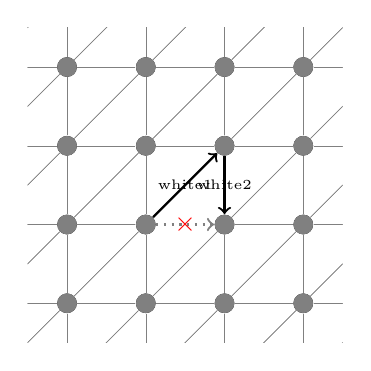
\begin{tikzpicture}
	
	%\clip (2.25cm,-0.5cm) rectangle +(3.25cm,3.0cm);
	\clip (2.5cm,1.5cm) rectangle +(4cm,4cm);
	
	\begin{scope}[minimum size=0.25cm,inner sep=0]
		\foreach \y in {-1,...,8}{
			\foreach \x in {-1,...,8}{
				\ifthenelse{\equal{\x\y}{43} \OR \equal{\x\y}{54} \OR \equal{\x\y}{53}}{
					\node (chip \x \y) at (\x,\y) [fill,circle] {};
				}{
					\node (chip \x \y) at (\x,\y) [fill=gray,circle] {};
				}
			}
		}
	\end{scope}
	
	\begin{scope}[help lines]
		\foreach \y in {0,...,7}{
			\foreach \x in {0,...,7}{
				\pgfmathtruncatemacro{\xx}{\x+1}
				\pgfmathtruncatemacro{\yy}{\y+1}
				\draw (chip \x \y) -- (chip \xx \yy);
				
				\pgfmathtruncatemacro{\xx}{\x-1}
				\pgfmathtruncatemacro{\yy}{\y-1}
				\draw (chip \x \y) -- (chip \xx \yy);
				
				\pgfmathtruncatemacro{\xx}{\x+1}
				\pgfmathtruncatemacro{\yy}{\y+0}
				\draw (chip \x \y) -- (chip \xx \yy);
				
				\pgfmathtruncatemacro{\xx}{\x-1}
				\pgfmathtruncatemacro{\yy}{\y+0}
				\draw (chip \x \y) -- (chip \xx \yy);
				
				\pgfmathtruncatemacro{\xx}{\x+0}
				\pgfmathtruncatemacro{\yy}{\y+1}
				\draw (chip \x \y) -- (chip \xx \yy);
				
				\pgfmathtruncatemacro{\xx}{\x+0}
				\pgfmathtruncatemacro{\yy}{\y-1}
				\draw (chip \x \y) -- (chip \xx \yy);
			}
		}
	\end{scope}
	
	% Hide existing link and redraw as dead link
	\draw [ultra thick, white] (chip 43) -- (chip 53);
	\draw [->, gray, thick, dotted]
	      (chip 43)
	   -- coordinate (dead link center)
	      (chip 53);
	\node [red] at (dead link center) {$\times$};
	
	% Draw emergency route 1
	\draw [ultra thick, white] (chip 43) -- (chip 54);
	\draw [->, thick]
	      (chip 43)
	   -- coordinate (first link center)
	      (chip 54);
	\node [font=\tiny] at (first link center) {\contour{white}{1}};
	
	% Draw emergency route 2
	\draw [ultra thick, white] (chip 54) -- (chip 53);
	\draw [->, thick]
	      (chip 54)
	   -- coordinate (second link center)
	      (chip 53);
	\node [font=\tiny] at (second link center) {\contour{white}{2}};
	
\end{tikzpicture}


			
			\caption{Connectivity between boards (circles) in a SpiNNaker system. A
			link undergoing a speed change is avoided by traversing two neighbouring
			links.  Wrap-around links are not shown.}
			\label{fig:emergency-routing}
		\end{figure}
		
		Two complementary approaches are being considered: the first involves
		transmitting data redundantly while a link is changing speed. During speed
		changes, the link becomes unreliable; existing systems simply wait until the
		link stabilises at the expense of latency To avoid adding additional
		hardware for this special case. In the proposed system, redundant
		transmission of data during link speed changes will be used. One possibility
		is the use of Forward Error Correction (FEC) \cite{hamming50} which allows
		errors to be corrected inexpensively. The second approach is to redirect
		data via an alternative route during link speed changes. This is possible
		because board-to-board links in SpiNNaker are also arranged in a 2D toroidal
		mesh meaning that while a link changes speeds, data can be redirected via
		two neighbouring links as shown in figure \ref{fig:emergency-routing}.
		
		Energy consumption will be measured using the benchmarks described above
		along with the power measurement techniques used by other researchers
		\cite{sharp12,stromatias13}.


\section{Conclusions}
	
	Large scale neural simulations represent a rich opportunity for
	neuroscientists to understand the brain but are held back by the computational
	expense of their execution. While specialised architectures such as SpiNNaker
	have significantly advanced the state of the art, their interconnection
	networks are only beginning to adopt the HSS interconnect technologies which
	have seen heavy investment by the super-computer industry \cite{infinibandta}.
	
	This work aims to develop a new generation of HSS-based networks for neural
	simulators which improve both system performance and power efficiency.
	Preliminary work has developed network modelling tools and proposed a novel
	technique which adds small-world connectivity to HSS networks capable of
	reducing both latency and network load. Planned work will implement this
	small-world connectivity scheme within SpiNNaker's HSS board-to-board
	interconnect and complement this with the development of a power management
	scheme for HSS links which is appropriate for neural systems.
